\documentclass[12pt]{article}

\usepackage[utf8x]{inputenc}%
\usepackage{graphicx}%
\usepackage{bibentry}%
\usepackage{hyperref}%
\usepackage{import}%
\usepackage{amsmath}%
\usepackage[romanian]{babel}%
\usepackage{color}%
\usepackage{algorithm}%
%\usepackage{algorithmic}%
\usepackage[noend]{algpseudocode}%
\usepackage{xfrac}
\usepackage{caption}
\usepackage{subcaption}
\usepackage{minted}%


\author{Tudor Berariu \\ \emph{tudor.berariu@gmail.com} \\ Laboratorul
  AI-MAS \\ Faculatea de Automatică și Calculatoare}
\title{Inteligență Artificială \\ Tema 2: \textbf{Planificare}}

\renewcommand{\algorithmicprocedure}{\textbf{Procedura}}
\renewcommand{\algorithmicwhile}{\textbf{cât timp}}
\renewcommand{\algorithmicdo}{\textbf{execută}}
\renewcommand{\algorithmicend}{\textbf{termină}}
\renewcommand{\algorithmicif}{\textbf{dacă}}
\renewcommand{\algorithmicthen}{\textbf{atunci}}
\renewcommand{\algorithmicelse}{\textbf{altfel}}

\definecolor{sapphire}{rgb}{0.03, 0.15, 0.4}
\newcommand{\repr}[1]{{\color{sapphire}\texttt{#1}}}
\definecolor{burntorange}{rgb}{0.8, 0.33, 0.0}
\newcommand{\racket}[0]{{\color{burntorange}\texttt{Racket}} }

\begin{document}

\maketitle

\section{Scopul temei}
\label{sec:scop}

\paragraph{}

Scopul acestei teme îl reprezintă familiarizarea cu conceptul de
planificare și implementarea unui algoritm pentru rezolvarea
planificării într-un mediu dinamic.

\paragraph{}

În continuare se prezintă o descriere generală a problemei ce trebuie
rezolvată (Secțiunea~\ref{sec:descriere}), a predicatelor folosite
pentru reprezentarea cunoștințelor depspre universul problemei
(Secțiunea~\ref{sec:reprezentare}), a operatorilor ce folosiți în
planificare (Secțiunea~\ref{sec:operatori}) și a planificatorului
robotului (Secțiunea~\ref{sec:planificator}).


\section{Problema celor doi roboți}
\label{sec:descriere}

\subsection{Descrierea problemei}
\label{sec:descriere}

\paragraph{Camerele și depozitele}

Pe un etaj al unei clădiri se află un labirint de camere cu uși
de acces între ele. Accesul nu este obligatoriu bidirecțional. Două
dintre acestea au o destinație specială, fiind depozite: camera roșie
și camera albastră. Restul camerelor sunt albe.

\paragraph{Sferele}

În aceste camere se află un număr de sfere de culoare roșie, albastră sau
gri.

\paragraph{Roboții}

La început atât în camera roșie, cât și în camera albastră, se află
câte un robot de aceeași culoare (roșu, respectiv albastru). Fiecare
dintre aceștia are misiunea de a aduce în depozitul propriu toate
sferele de aceeași culoare (vezi Figura~\ref{fig:exemplu}).

\begin{figure}[h!]
  \centering
  \begin{subfigure}[b]{0.48\textwidth}
    \includegraphics[width=\textwidth]{graphics/start.pdf}
    \caption{Configurația de start}
    \label{fig:start}
  \end{subfigure}
  \begin{subfigure}[b]{0.48\textwidth}
    \includegraphics[width=\textwidth]{graphics/final.pdf}
    \caption{O posibilă stare finală}
    \label{fig:final}
  \end{subfigure}
  \caption{Exemplu de scenariu (camerele și ușile sunt reprezentate
    prin noduri și arce în graf)}
  \label{fig:exemplu}
\end{figure}

\paragraph{}

Fiecare dintre roboți se poate deplasa liber dintr-o cameră în oricare
altă cameră vecină către care există acces. Fiecare dintre roboți are 2 spații
interne de depozitare în care poate încărca câte o sferă indiferent de
culoare. Deoarece aceste sfere sunt destul de grele, iar
compartimentele se află în părțile laterale ale robotului, acesta nu
se poate deplasa dintr-o cameră în alta cu un singur compariment
încărcat. Așadar, robotul se poate muta, fie cu ambele spații interne
de stocare goale, fie cu ambele încărcate cu câte o sferă. Un robot
poate încărca și descărca orice sferă din și în orice cameră cu o
singură excepție: nu se pot încărca sferele aflate deja în depozitul
lor (sferele duse în depozitul lor nu mai pot fi mișcate).

\paragraph{Misiunea}

Pe etaj sunt $N$ camere (depozitul roșu, depozitul albastru și $N-2$
camere albe), $M$ sfere roșii, $M$ sfere albastre și $N$ sfere gri
(inițial câte o sferă gri în fiecare cameră, vezi
Figura~\ref{fig:start}). Un robot își încheie misiunea atunci când
toate cele $M$ sfere de aceeași culoare se află în depozitul
corespunzător. Poziția finală a sferelor gri nu este importantă.

\paragraph{}

Mutarea dintr-o cameră într-o altă cameră vecină, încărcarea unei
sfere și descărcarea unei sfere se fac într-o unitate de timp. De
asemenea, procesul care constă în actualizarea informațiilor despre
pozițiile tuturor sferelor din toate camerele și conceperea unui plan
(o secvență de acțiuni) necesită o unitate de timp. Cum robotul
acționează într-un mediu dinamic, se poate întâmpla ca până la
momentul aplicării unei operator, condițiile acestuia să nu mai fie
adevărate. Dacă robotul încearcă să execute o acțiune ce nu se poate
aplica (de exemplu: încărcarea unei sfere care nu se găsește în camera
curentă), atunci acesta se blochează și mai are nevoie de o unitate de
timp pentru a-și reveni. Aplicarea unui operator eronat (de exemplu:
încărcarea unei a treia sfere, mutarea dintr-o cameră în alta care nu
este vecină cu prima, etc.) se penalizează de asemenea prin blocarea
robotului pentru o unitate de timp. După ce se deblochează, reintră în
rutina de planificare.

\paragraph{}

Se caută ingineri care să programeze un planificator pentru acești doi
roboți astfel încât aceștia să rezolve cât mai repede misiunea pe care
au.

\subsection{Reprezentarea cunoștințelor}
\label{sec:reprezentare}

\paragraph{Convenție}

Vom folosi nume cu litere mici pentru a ne referi la constante
(e.g. \repr{room1}, \repr{blue}) și nume ce încep cu litere mari
pentru a ne referi la variabile (\repr{Room}, \repr{Color}). De
asemenea, vom folosi nume ce încep cu literă mică pentru a ne referi
la predicate (e.g. \repr{spheres($\cdot$, $\cdot$, $\cdot$)}) și nume
cu litere mari pentru a ne referi la operatori
(e.g. \repr{Move($\cdot$)}).

\paragraph{}

Pentru a reprezenta cunoștințele despre mediu se vor folosi
predicatele:
\begin{itemize}
\item \repr{location(Room)} - cu semnificația că robotul se află în
  camera \repr{Room};
\item \repr{spheres(Color, Room, N)} - cu semnificația că în camera
  \repr{Room} se găsesc \repr{N} sfere de culoarea \repr{Color};
\item \repr{color(Room, Color)} - cu semnificația că încăperea
  \repr{Room} are culoarea \repr{Color};
\item \repr{color(Color)} - cu semnificația că robotul are culoarea
  \repr{Color};
\item \repr{door(Room1, Room2)} - cu semnificația că se poate trece
  din camera \repr{Room1} în camera \repr{Room2};
\item \repr{carries(Color, N)} - cu semnificația că robotul are
  încărcate în compartimentele interne \repr{N} sfere de culoarea
  \repr{Color}.
\item \repr{succ(N1, N2)} - predicat ce va fi adevărat pentru orice
  numere naturale \repr{N1} și \repr{N2} consecutive (\repr{N2 =
    N1 + 1});
\item \repr{greater(N1, N2)} - predicat ce va fi adevărat pentru
  orice numere naturale \repr{N1} și \repr{N2} pentru care
  (\repr{N1 $>$ N2});
\item \repr{positive(N)} - predicat ce va fi adevărat pentru orice
  număr natural strict pozitiv \repr{N}.
\end{itemize}

\paragraph{}

Intern robotul poate folosi oricâte alte predicate pentru a reprezenta
complet starea sa sau pe cea a mediului, însă doar cele enumerate mai
sus vor fi folosite pentru a transmite starea curentă planificatorului
atât la începutul programului, cât și pe parcurs când este necesară
replanificarea.

\subsection{Operatori}
\label{sec:operatori}

\paragraph{}

Planurile conțin următoarii operatori:
\begin{itemize}
\item \repr{Move(Room1, Room2)} care reprezintă acțiunea prin care
  agentul se mută din camera \repr{Room1} în camera \repr{Room2}.
  Acțiunea \repr{Move} reușește doar dacă există o ușă între
  \repr{Room1} și \repr{Room2} și, fie ambele compartimente ale
  robotului sunt pline, fie ambele compartimente sunt goale (robotul
  cară zero sau două sfere).
\item \repr{Load(Color)} care reprezintă acțiunea prin care agentul
  culege o sferă de culoarea \repr{Color} din camera în care se află
  și-o încarcă într-un spațiu intern de stocare liber. Acțiunea
  reușește întotdeauna dacă în camera în care se află agentul există
  cel puțin o sferă de culoare \repr{Color}, camera nu are aceeași
  culoare cu sfera și robotul nu cară deja două sfere.
\item \repr{Unload(Color)} care reprezintă acțiunea prin care
  agentul descarcă o sferă de culoare \repr{Color} în camera în care
  se află. Acțiunea reușește numai dacă robotul are în compartimentele
  interne cel puțin o sferă de culoare \repr{Color}.
\end{itemize}

Fiecare dintre acești operatori se execută într-o unitate de timp.

\paragraph{}

Mai există un operator special, \repr{Test($\cdot$)}, care îi permite
robotului să verifice informații despre lumea înconjurătoare.

\begin{itemize}
\item \repr{Test(Condition)} a cărui aplicare constă în verificarea
  conjuncției de predicate din \repr{Condition}. În cazul în care
  condițiile sunt adevărate, planul este continuat prin aplicarea
  următoarei acțiuni, altfel, se abandonează planul curent pentru
  replanificare.\\
  \repr{Condition} poate conține doar predicatele \repr{spheres},
  \repr{succ}, \repr{greater} și \repr{positive} (restul informațiilor
  despre lume nu se schimbă pe parcurs). De exemplu, pentru a verifica
  faptul că în \repr{room1} se găsesc cel puțin două bile roșii:
  \begin{center}
    \repr{spheres(red, room1, N1)} $\wedge$ \repr{succ(N1, N)}
    $\wedge$ \repr{positive(N)}
  \end{center}
  sau, pentru a verifica simultan că în camera \repr{room1} se află cu
  cel puțin două sfere roșii mai multe decât în camera \repr{room2},
  iar în camera \repr{room3} se află o singură sferă gri (de data
  aceasta în sintaxă \racket):
  \begin{minted}[]{racket}
    ((spheres red room1 N1) (spheres red room2 N2) (succ N N1)
    (greater N N2) (spheres grey room3 1))
  \end{minted}
\end{itemize}

\subsection{Planificatorul}
\label{sec:planificator}

\paragraph{}

Planificatorul robotului \textbf{nu} are memorie internă. El primește
patru informații:
\begin{itemize}
\item obiectivul său, un predicat de forma
  \repr{spheres(Color,Warehouse,M)} (e.g., pentru robotul
  roșu: \repr{spheres(red, redWarehouse, m)});
\item starea lumii: culoarea lui, camera în care se află el, numărul
  de sfere de culoare gri, roșie și albastră din fiecare cameră,
  perechile de camere vecine și culorile camerelor;
\item restul de acțiuni ce nu au fost executate, dacă a eșuat
  aplicarea unui plan sau verificarea condiției unui operator
  \repr{Test};
\item o listă cu informații suplimentare, pe care robotul a reîntors-o
  odată cu ultimul plan (permite salvarea unui context de calcul și
  simulează memoria internă).
\end{itemize}

Rezultatul planificării conține 2 elemente:
\begin{itemize}
\item planul efectiv: o secvență de operatori dintre \repr{Move},
  \repr{Load}, \repr{Unload} și \repr{Test};
\item o listă conținând orice informații; aceasta îi va fi retrimisă
  planificatorului dacă planul eșuează sau verificarea condiției unui
  operator \repr{Test} eșuează.
\end{itemize}


\section{Cerințe}
\label{sec:tasks}

\subsection{[0.3p] Cerința 1: Descriere STRIPS}

\paragraph{}

Folosind predicatele enumerate în secțiunea anterioară, dar și alte
predicate suplimentare pe care le considerați necesare, descrieți
următorii operatori folosind STRIPS: \repr{Move}, \repr{Load} și
\repr{Unload}.

\paragraph{}

Operatorul \repr{Test} are un statut special și nu trebuie descris.

\subsection{[0.7p] Cerința 2: Planificare simplă}

\paragraph{}

Să se implementeze un planificator \repr{memoryless-agent} care
construiește planuri pentru aducerea unei sfere în
depozit. Planificatorul va fi folosit astfel:

\begin{algorithm}[H]
  \caption{Funcționarea robotului}\label{alg:robot}
  \begin{algorithmic}[1]
    \While{mai sunt bile de adus}
    \State $p \leftarrow$ \repr{memoryless-agent(goal, world-state)}
    \While{planul $p$ mai conține operatori}
    \State $o_1 \leftarrow pop(p)$
    \If{se poate aplica $o_1$}
    \State execută $o_1$
    \Else
    \State întrerupe execuția planului
    \EndIf
    \EndWhile
    \EndWhile
  \end{algorithmic}
\end{algorithm}

Cât timp mai există bile de adus în depozit, planificatorul este
folosit pentru construirea unui plan care să aducă următoarea sferă în
depozit. Atât timp cât se pot aplica operatorii planului, aceștia sunt
executați. Dacă la un moment dat o acțiune nu poate fi aplicată,
robotul se blochează pentru o unitate de timp și trebuie să
replanifice.

\paragraph{}

Se poate alege orice strategie de planificare pentru rezolvarea
acestei cerințe (căutare înainte, căutare înapoi, altceva).

\paragraph{}

Agentul \repr{memoryless-agent} nu poate include operatorul
\repr{Test} în planul lui și nici nu-și poate salva informații pe
care să le utilizeze în momentul replanificării.

\paragraph{}

Planificatorul agentului \repr{memoryless-agent} va fi apelat de
fiecare dată astfel:
\begin{center}
  \repr{(memoryless-agent goal world-state null null)}.
\end{center}
unde \repr{goal} va fi \repr{(spheres Color Warehouse (+ 1 M))},
\repr{Color} este culoarea robotului, \repr{Warehouse} reprezintă
depozitul, iar \repr{M} este numărul de bile duse deja acolo.

Agentul nu va face diferența între o planificare de la zero și o
replanificare după eșecul aplicării unui operator.

\paragraph{}

Testarea se va face folosind planificatorul \repr{memoryless-agent}
atât pentru agentul roșu și \repr{dummy-agent} sau
\repr{memoryles-agent} pentru cel albastru.

\begin{minted}[]{racket}
  (run scenario4 memoryless-agent dummy-agent)
\end{minted}

\begin{minted}[]{racket}
  (run scenario2 memoryless-agent memoryless-agent)
\end{minted}


\paragraph{Recomandare pentru o implementare frumoasă}

Încercați să construiți un planificator care să funcționeze
independent de problema dată (separați algoritmul care construiește
planul de detalii ce țin de problema descrisă).

\subsection{[BONUS 0.2p] Cerința 3: Tehnici de planificare avansată}

\paragraph{}

Să se implementeze un agent \repr{advanced-agent} care este mai
eficient decât \repr{memoryless-agent}. Se poate folosi orice
strategie pentru căutarea / construirea planului. Mai mult, agentul
poate include în acțiunile din plan operatorul
\repr{Test(Condition)}, unde \repr{Condition} este o listă
predicate dintre \repr{spheres}, \repr{succ}, \repr{greater} și
\repr{positive}. Dacă acestea nu sunt adevărate în starea curentă,
se apelează funcția:
\begin{center}
  \repr{(advanced-agent goal world-state rest-of-actions
    saved-info)}.
\end{center}

\paragraph{}

Pentru a da mai multe posibilități de implementare,
\repr{advanced-agent} va primi întotdeauna un singur obiectiv: starea
în care toate sferele se află în depozit.

\paragraph{}

Sarcina acestei cerințe este de a construi un planificator cât mai
eficient. Se recomandă exploatarea următoarelor direcții:
\begin{itemize}
\item optimizarea căutării planului prin folosirea unei euristici care
  să o ghideze;
\item repararea unui plan eșuat fără a reface replanificarea de la
  zero (vezi Figura~\ref{fig:repair});
\item gestionarea simultană a mai multor planuri.
\end{itemize}

\begin{figure}[h!]
  \centering
  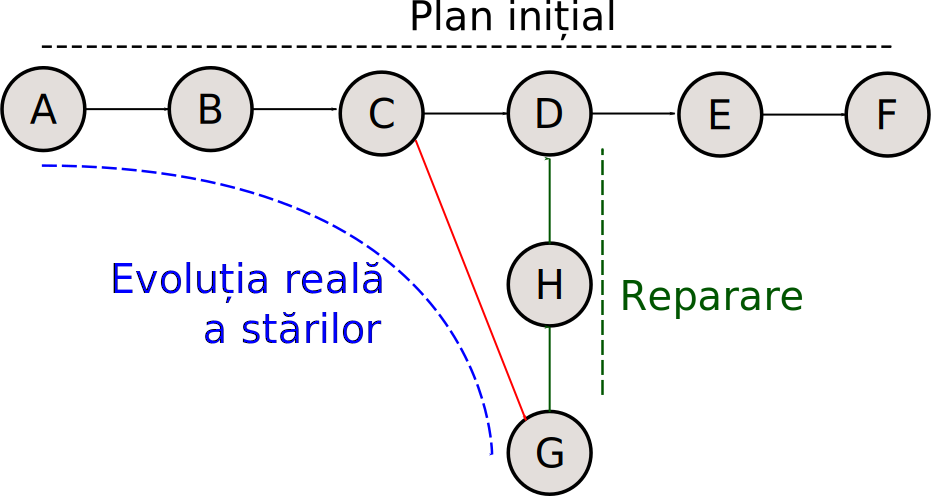
\includegraphics[width=.5\textwidth]{graphics/replan.pdf}
  \caption{Replanificare: repararea unui plan}
  \label{fig:repair}
\end{figure}

În Figura~\ref{fig:repair} este reprezentat un plan inițial care
într-un mediu static ar fi dus la secvența de stări: $A \rightarrow B
\rightarrow C \rightarrow D \rightarrow E \rightarrow F$. Cum însă
mediul este unul dinamic, din starea $C$ s-a ajuns în starea $G$
(tranziția marcată cu roșu). Repararea unui plan presupune găsirea
unei secvențe de acțiuni care să ducă mediul înapoi în starea $D$ de
unde să se reia restul de acțiuni din planul inițial. Practic
replanificarea va produce un plan $G \rightarrow H \rightarrow D
\rightarrow E \rightarrow F$ realizat prin concatenarea planului de
reparare cu restul planului precedent.

\paragraph{}

Testarea \repr{advanced-agent} se va face prin plasarea lui în același
scenariu cu \repr{memoryless-agent} (primul va fi planificatorul
robotului roșu, iar celălalt planificatorul robotului albastru). Se va
adăuga un al patrulea parametru funcției \repr{run}, \repr{\#t}.

\begin{minted}[]{racket}
  (run scenario4 advanced-agent memoryless-agent #t)
\end{minted}

\section{Trimiterea temei}
\label{sec:send}

\paragraph{}

Cerința 1 se trimite într-un fișier pdf:
\begin{center}
  \texttt{Nume\_Prenume\_Grupa\_IA\_T2.pdf}
\end{center}

\paragraph{}

Cerințele 2 și 3 se completează în fișierul \racket atașat
(\texttt{planning.rkt}) unde trebuie implementate funcțiile
\repr{memoryless-agent} și [opțional] \repr{advanced-agent}. Așa
cum s-a discutat mai sus, fiecare dintre acestea primește 4 parametri:
\begin{enumerate}
\item \repr{goals} - un predicat reprezentând obiectivul robotului;
\item \repr{world-state} - listă de predicate care descrie starea
  lumii (culoarea robotului, camera în care se află, culorile tuturor
  camerelor, ușile dintre camere, numărul de sfere din fiecare culoare
  din fiecare cameră);
\item \repr{left-actions} - listă de acțiuni ce au rămas neexecutate
  din planul precedent [doar pentru \repr{advanced-agent}];
\item \repr{info} - valoarea pe care a reîntors-o aceeași funcție
  odată cu planul precedent (memoria) [doar pentru
  \repr{advanced-agent}];
\end{enumerate} și reîntorc o pereche \repr{(plan . info)} unde
\repr{plan} este o listă de acțiuni, iar \repr{info} poate lua orice
valoare.

Acțiunile vor fi liste în care pe prima poziție se regăsește numele
operatorului, urmat de argumentele acestuia (obiecte din lumea
problemei).

\paragraph{}

Pentru cerințele 2 și 3 se vor adăuga câteva explicații în fișierul
pdf:
\begin{itemize}
\item algoritmul ales pentru planificare;
\item comparații între agenții implementați.
\end{itemize}

\section{Scenarii de test}
\label{sec:test}

În fișierul \texttt{planning.rkt} sunt definite șase scenarii:
\repr{scenario0}, $\ldots$, \repr{scenario5}.

\begin{figure}[h!]
  \centering
  \includegraphics[width=0.66\textwidth]{graphics/scenario0.pdf}
  \caption{Starea inițială pentru scenariul 0}
  \label{fig:s0}
\end{figure}

\begin{figure}[h!]
  \centering
  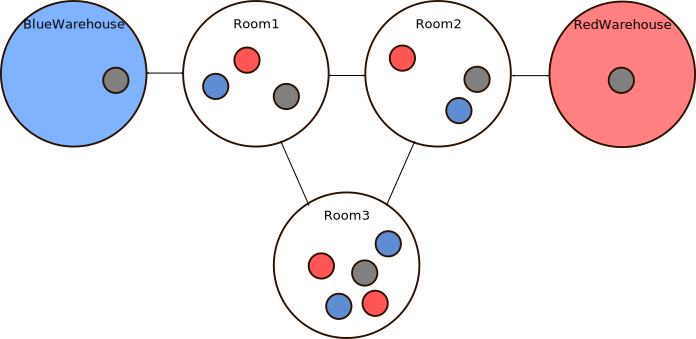
\includegraphics[width=0.66\textwidth]{graphics/scenario1.pdf}
  \caption{Starea inițială pentru scenariul 1}
  \label{fig:s1}
\end{figure}

\begin{figure}[h!]
  \centering
  \includegraphics[width=0.66\textwidth]{graphics/scenario2.pdf}
  \caption{Starea inițială pentru scenariul 2}
  \label{fig:s2}
\end{figure}


\begin{figure}[h!]
  \centering
  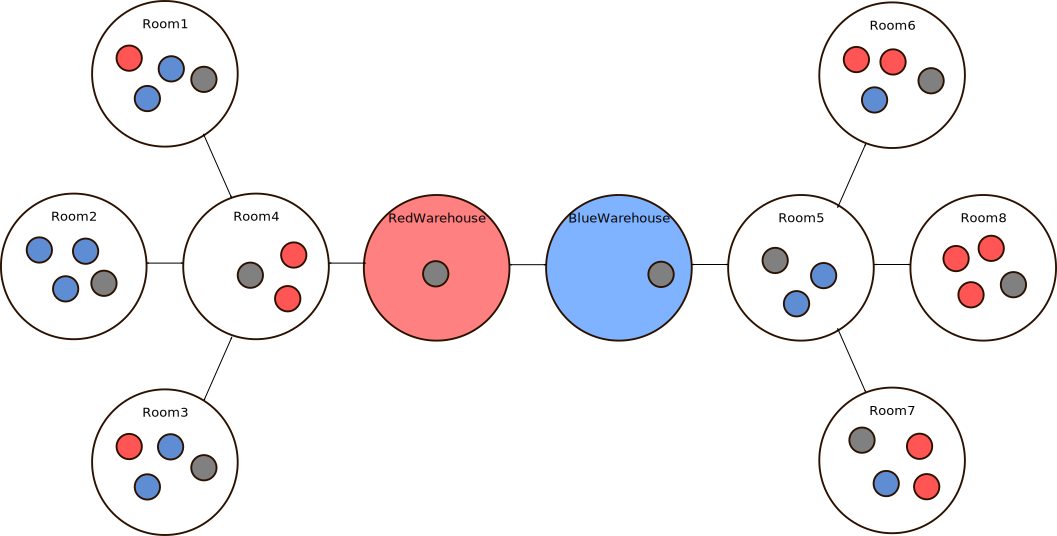
\includegraphics[width=\textwidth]{graphics/scenario3.pdf}
  \caption{Starea inițială pentru scenariul 3}
  \label{fig:s3}
\end{figure}

\begin{figure}[h!]
  \centering
  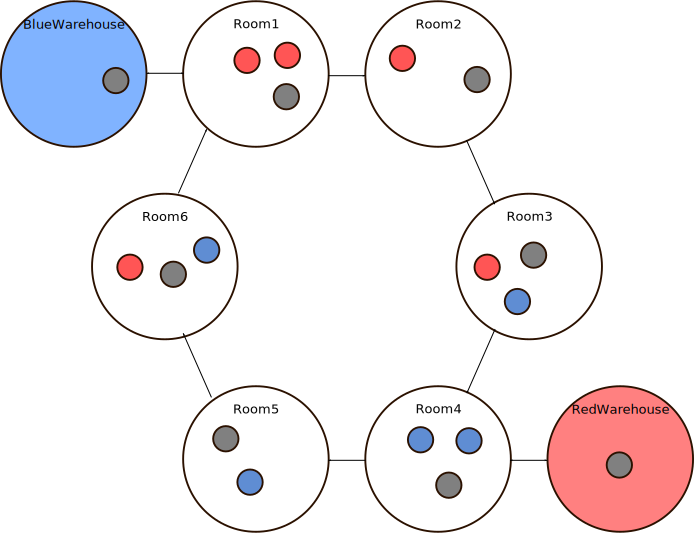
\includegraphics[width=0.66\textwidth]{graphics/scenario4.pdf}
  \caption{Starea inițială pentru scenariul 4}
  \label{fig:s4}
\end{figure}

\begin{figure}[h!]
  \centering
  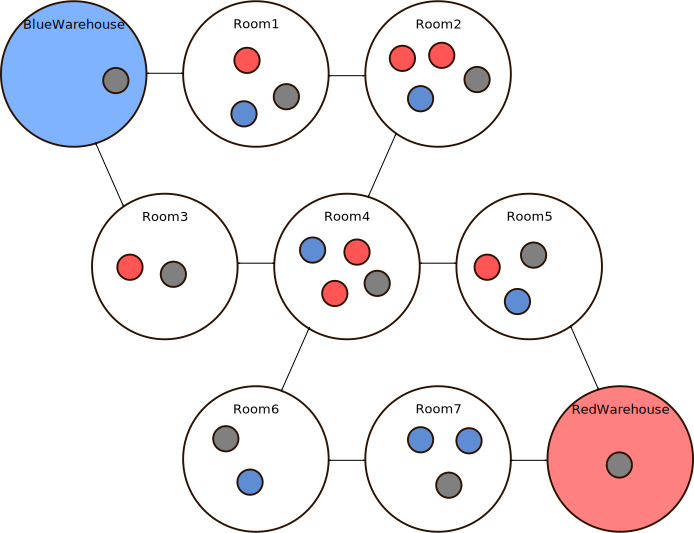
\includegraphics[width=0.66\textwidth]{graphics/scenario5.pdf}
  \caption{Starea inițială pentru scenariul 5}
  \label{fig:s5}
\end{figure}


\end{document}
